\documentclass[aspectratio=169,10pt]{beamer}

% Theme selection
\usetheme{AnnArbor}
\usecolortheme{dolphin}

% Font and encoding for Vietnamese
\usepackage{fontspec}
\setmainfont{DejaVu Sans}
\setsansfont{DejaVu Sans}
\setmonofont{Consolas}

\usepackage{booktabs}
\usepackage{array}
\usepackage{tabularx}
\usepackage{listings}
\usepackage{tikz}
\usepackage{amsmath}
\usepackage{amssymb}
\usepackage{adjustbox}
\usetikzlibrary{shapes,arrows,positioning,calc}

% Color definitions
\definecolor{codegray}{rgb}{0.95,0.95,0.95}
\definecolor{codeblue}{rgb}{0.1,0.2,0.6}
\definecolor{codegreen}{rgb}{0.1,0.5,0.1}
\definecolor{crimsonred}{rgb}{0.8,0.1,0.1}
\definecolor{darkgreen}{rgb}{0.0,0.4,0.0}
\definecolor{accentorange}{rgb}{0.85,0.4,0.0}

% Custom code style
\newcommand{\code}[1]{\texttt{\textcolor{codeblue}{#1}}}

% Slide Metadata
\title[Phân cụm Dữ liệu (Clustering)]{\Large \textbf{CHUYÊN ĐỀ: PHÂN CỤM DỮ LIỆU TRONG MACHINE LEARNING}}
\subtitle{\normalsize Lý Thuyết Toàn Diện, Ý Nghĩa Công Thức, Ví Dụ Tính Tay, Ứng Dụng Thực Tế \& Cẩm Nang Lựa Chọn}
\author[TS. Vũ Đức Minh]{TS. Vũ Đức Minh}
\institute[NEU]{Khoa Khoa học Dữ liệu và Trí tuệ Nhân tạo\\Trường Công nghệ -- Đại học Kinh tế Quốc dân (NEU)}
\date{2026}

\begin{document}

% Slide 1: Title
\begin{frame}
  \titlepage
\end{frame}

% Slide 2: Mục tiêu bài giảng
\begin{frame}{Mục tiêu Bài học (Learning Objectives)}
  \small
  \begin{itemize}\setlength{\itemsep}{2.5pt}
    \item \textbf{Bản chất Phân cụm (Clustering):} Hiểu rõ triết lý Học không giám sát (Unsupervised Learning) và phân biệt \textbf{Hard Clustering} vs \textbf{Soft Clustering}.
    \item \textbf{Ý nghĩa Công thức \& Độ đo Khoảng cách:} Hiểu trực giác toán học của WCSS, Linkage criteria, Mật độ $\varepsilon$-neighborhood, Định lý Bayes trong EM, và Hệ số Silhouette.
    \item \textbf{Làm chủ 5 trường phái thuật toán cốt lõi qua Ví dụ Tính tay:}
      \begin{enumerate}\setlength{\itemsep}{1.5pt}
        \item \textbf{Centroid-based:} K-Means, K-Means++, Elbow Method, K-Medoids.
        \item \textbf{Connectivity-based:} Hierarchical Clustering, Dendrogram, 5 Linkage Criteria.
        \item \textbf{Density-based:} DBSCAN (Core/Border/Noise), OPTICS (Reachability Plot).
        \item \textbf{Distribution-based:} Gaussian Mixture Models (GMM), Thuật toán EM.
        \item \textbf{Fuzzy Clustering:} Fuzzy C-Means (FCM) với độ thuộc mờ $u_{ik}$.
      \end{enumerate}
    \item \textbf{Ứng dụng Thực tế Đột phá:} Nắm bắt các bài toán lớn trong E-commerce, Y sinh học, Ngân hàng chống gian lận, Định vị GPS và Xử lý tiếng nói.
    \item \textbf{Cẩm nang Lựa chọn Thuật toán:} Làm chủ ma trận kịch bản kinh doanh và kỹ thuật để chọn đúng mô hình phân cụm cho từng bài toán thực tế.
  \end{itemize}
\end{frame}

% Slide 3: Tổng quan Unsupervised Learning & Clustering
\begin{frame}{1. Bản chất của Phân cụm Dữ liệu (Clustering)}
  \begin{columns}[T]
    \begin{column}{0.55\textwidth}
      \textbf{Khái niệm nền tảng (GeeksforGeeks):}
      \begin{itemize}\setlength{\itemsep}{2pt}
        \item Là bài toán trung tâm của \textbf{Học không giám sát (Unsupervised Learning)}.
        \item Dữ liệu đầu vào chỉ có các biến đặc trưng $\mathcal{X} = \{x_1, \dots, x_N\}$, \textbf{không có nhãn mục tiêu} $y$.
        \item \textbf{Mục tiêu tối thượng:} Tự động gom các quan sát vào các nhóm (cụm) sao cho:
          \begin{itemize}\setlength{\itemsep}{1pt}
            \item \textbf{Độ tương đồng nội cụm cao nhất} (High intra-cluster similarity).
            \item \textbf{Độ phân tách ngoại cụm lớn nhất} (High inter-cluster dissimilarity).
          \end{itemize}
        \item Cụm là tập hợp các điểm có hành vi, hình thái hoặc khoảng cách tương đồng.
      \end{itemize}
    \end{column}
    \begin{column}{0.45\textwidth}
      \begin{center}
        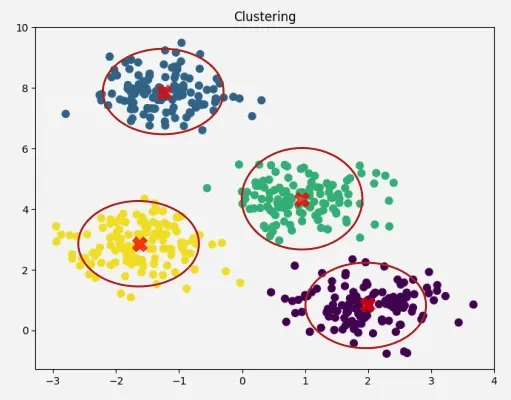
\includegraphics[width=0.95\linewidth,height=0.65\textheight,keepaspectratio]{images/clustering-overview.png}
      \end{center}
    \end{column}
  \end{columns}
\end{frame}

% Slide 4: Hard vs Soft Clustering
\begin{frame}{Phân loại Hình thức: Hard Clustering vs Soft Clustering}
  \begin{columns}[T]
    \begin{column}{0.52\textwidth}
      \textbf{1. Phân cụm cứng (Hard Clustering):}
      \begin{itemize}\setlength{\itemsep}{2pt}
        \item Mỗi điểm $x_i$ thuộc duy nhất về một cụm $C_k$ với xác suất tuyệt đối $100\%$.
        \item Nhãn phân cụm nhị phân: $z_{ik} \in \{0, 1\}$ thỏa mãn $\sum_{k=1}^K z_{ik} = 1$.
        \item \textit{Đại diện tiêu biểu:} K-Means, Hierarchical, DBSCAN.
      \end{itemize}
      \vspace{0.4em}
      \textbf{2. Phân cụm mềm (Soft / Fuzzy Clustering):}
      \begin{itemize}\setlength{\itemsep}{2pt}
        \item Mỗi điểm thuộc về tất cả các cụm với một \textbf{trọng số xác suất} hoặc mức độ thuộc (membership) $\gamma_{ik} \in [0, 1]$ thỏa mãn $\sum_{k=1}^K \gamma_{ik} = 1$.
        \item \textit{Đại diện tiêu biểu:} GMM (EM), Fuzzy C-Means (FCM).
      \end{itemize}
    \end{column}
    \begin{column}{0.48\textwidth}
      \begin{center}
        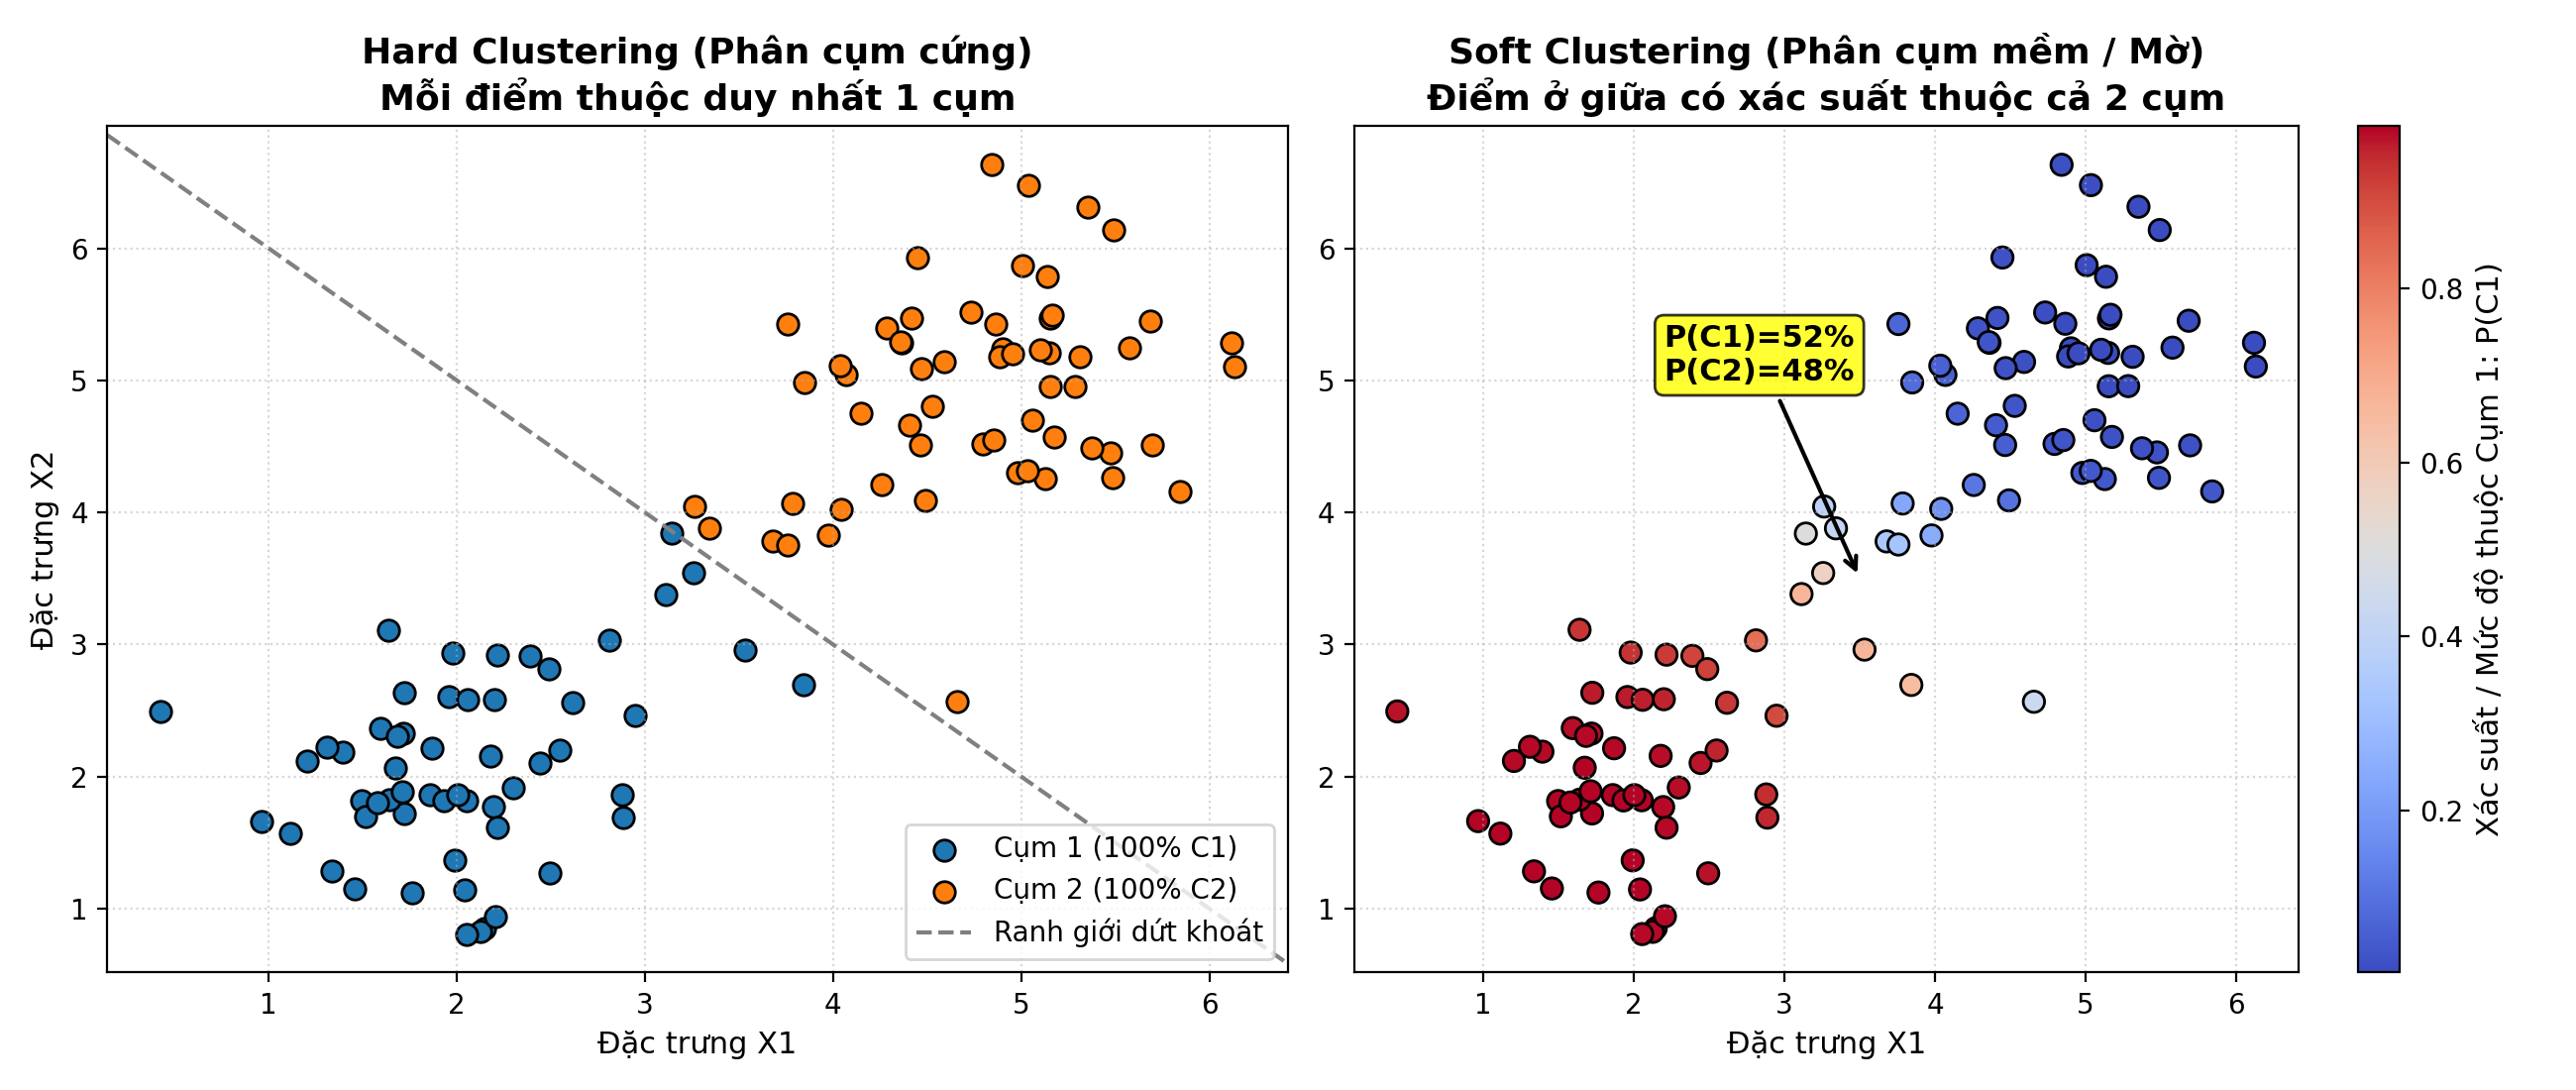
\includegraphics[width=0.98\linewidth,height=0.65\textheight,keepaspectratio]{images/hard-vs-soft-clustering.png}
      \end{center}
    \end{column}
  \end{columns}
\end{frame}

% Slide 5: Độ đo khoảng cách và độ tương đồng
\begin{frame}{Các Độ đo Khoảng cách \& Vai trò của Chuẩn hóa Dữ liệu}
  \small
  \begin{columns}[T]
    \begin{column}{0.52\textwidth}
      \textbf{Các hàm khoảng cách thông dụng:}
      \begin{itemize}\setlength{\itemsep}{2pt}
        \item \textbf{Euclidean Distance ($L_2$ norm):}
          $$d(x, z) = \sqrt{\sum_{j=1}^d (x_j - z_j)^2}$$
          Chuẩn mực cho biến định lượng liên tục cùng thang đo.
        \item \textbf{Manhattan Distance ($L_1$ norm / City Block):}
          $$d(x, z) = \sum_{j=1}^d |x_j - z_j|$$
          Bền vững hơn trước outliers, phù hợp không gian lưới.
        \item \textbf{Cosine Similarity (Góc vector):}
          $$\cos(\theta) = \frac{x \cdot z}{\|x\|_2 \|z\|_2}$$
          Chuẩn mực cho văn bản (TF-IDF), hệ gợi ý.
      \end{itemize}
    \end{column}
    \begin{column}{0.48\textwidth}
      \begin{center}
        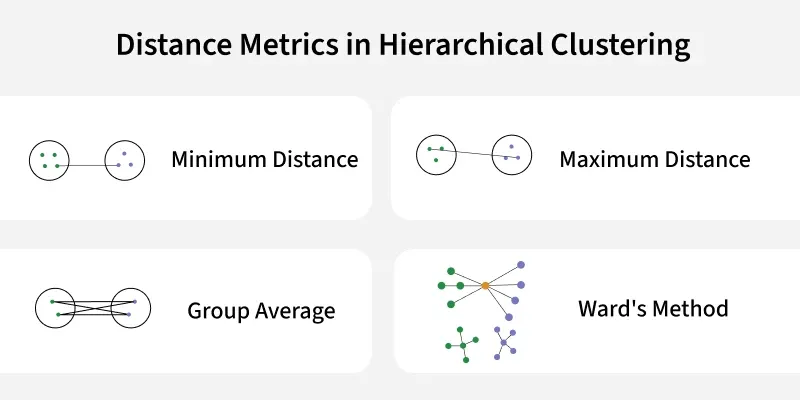
\includegraphics[width=0.98\linewidth,height=0.38\textheight,keepaspectratio]{images/distance-metrics.png}
      \end{center}
      \footnotesize
      \textbf{Lưu ý sống còn:} Phải thực hiện \textbf{Chuẩn hóa dữ liệu (StandardScaler)} trước khi tính khoảng cách, nếu không biến có giá trị lớn (ví dụ: Thu nhập $10^7$) sẽ áp đảo hoàn toàn biến nhỏ (Tuổi $10^1$)!
    \end{column}
  \end{columns}
\end{frame}

% Slide 6: Bức tranh toàn cảnh 5 trường phái
\begin{frame}{Bức tranh Toàn cảnh: 5 Trường phái Phân cụm Chính}
  \begin{table}[]
    \scriptsize
    \centering
    \begin{tabularx}{\textwidth}{l p{2.6cm} p{2.6cm} X}
      \toprule
      \textbf{Trường phái} & \textbf{Triết lý Gom cụm} & \textbf{Thuật toán Tiêu biểu} & \textbf{Đặc trưng Hình học} \\
      \midrule
      \textbf{Centroid-based} & Đại diện cụm bằng một tâm điểm trung tâm & K-Means, K-Means++, K-Medoids & Hình cầu lồi (Spherical), ô Voronoi \\
      \addlinespace
      \textbf{Connectivity} & Dựa trên khoảng cách lân cận giữa các mẫu & Agglomerative, Divisive, BIRCH & Cây phân cấp đa tầng (Dendrogram) \\
      \addlinespace
      \textbf{Density-based} & Cụm là vùng mật độ cao cách biệt bởi vùng thưa & DBSCAN, OPTICS, HDBSCAN & Hình dạng tùy ý, tự động lọc nhiễu \\
      \addlinespace
      \textbf{Distribution} & Dữ liệu sinh ra từ tổ hợp các phân phối xác suất & Gaussian Mixture Model (GMM), EM & Hình Elip tự do, xác suất thành viên mềm \\
      \addlinespace
      \textbf{Fuzzy / Mờ} & Điểm thuộc về cụm theo mức độ mờ ($u_{ik} \in [0,1]$) & Fuzzy C-Means (FCM) & Cụm giao thoa, đường biên mờ \\
      \bottomrule
    \end{tabularx}
  \end{table}
\end{frame}

% Slide 7: Centroid-based - K-Means
\begin{frame}{2. Centroid-based: Thuật toán K-Means Cổ điển}
  \small
  \begin{columns}[T]
    \begin{column}{0.55\textwidth}
      \textbf{Quy trình 4 bước của Lloyd (1957):}
      \begin{enumerate}\setlength{\itemsep}{1pt}
        \item \textbf{Khởi tạo:} Chọn ngẫu nhiên $K$ tâm cụm $\mu_1, \dots, \mu_K$.
        \item \textbf{Gán cụm (Assignment):} Gán mỗi điểm $x_i$ vào cụm có tâm gần nhất:
          $$c^{(i)} = \arg\min_k \|x_i - \mu_k\|_2^2$$
        \item \textbf{Cập nhật tâm (Update):} Tính lại toạ độ trọng tâm:
          $$\mu_k = \frac{1}{|C_k|} \sum_{x_i \in C_k} x_i$$
        \item \textbf{Lặp lại} bước 2 và 3 cho đến khi tâm không đổi.
      \end{enumerate}
      \textbf{Hàm mục tiêu (WCSS / Inertia):}
      $$J = \sum_{k=1}^K \sum_{x_i \in C_k} \|x_i - \mu_k\|_2^2 \to \min$$
    \end{column}
    \begin{column}{0.45\textwidth}
      \begin{center}
        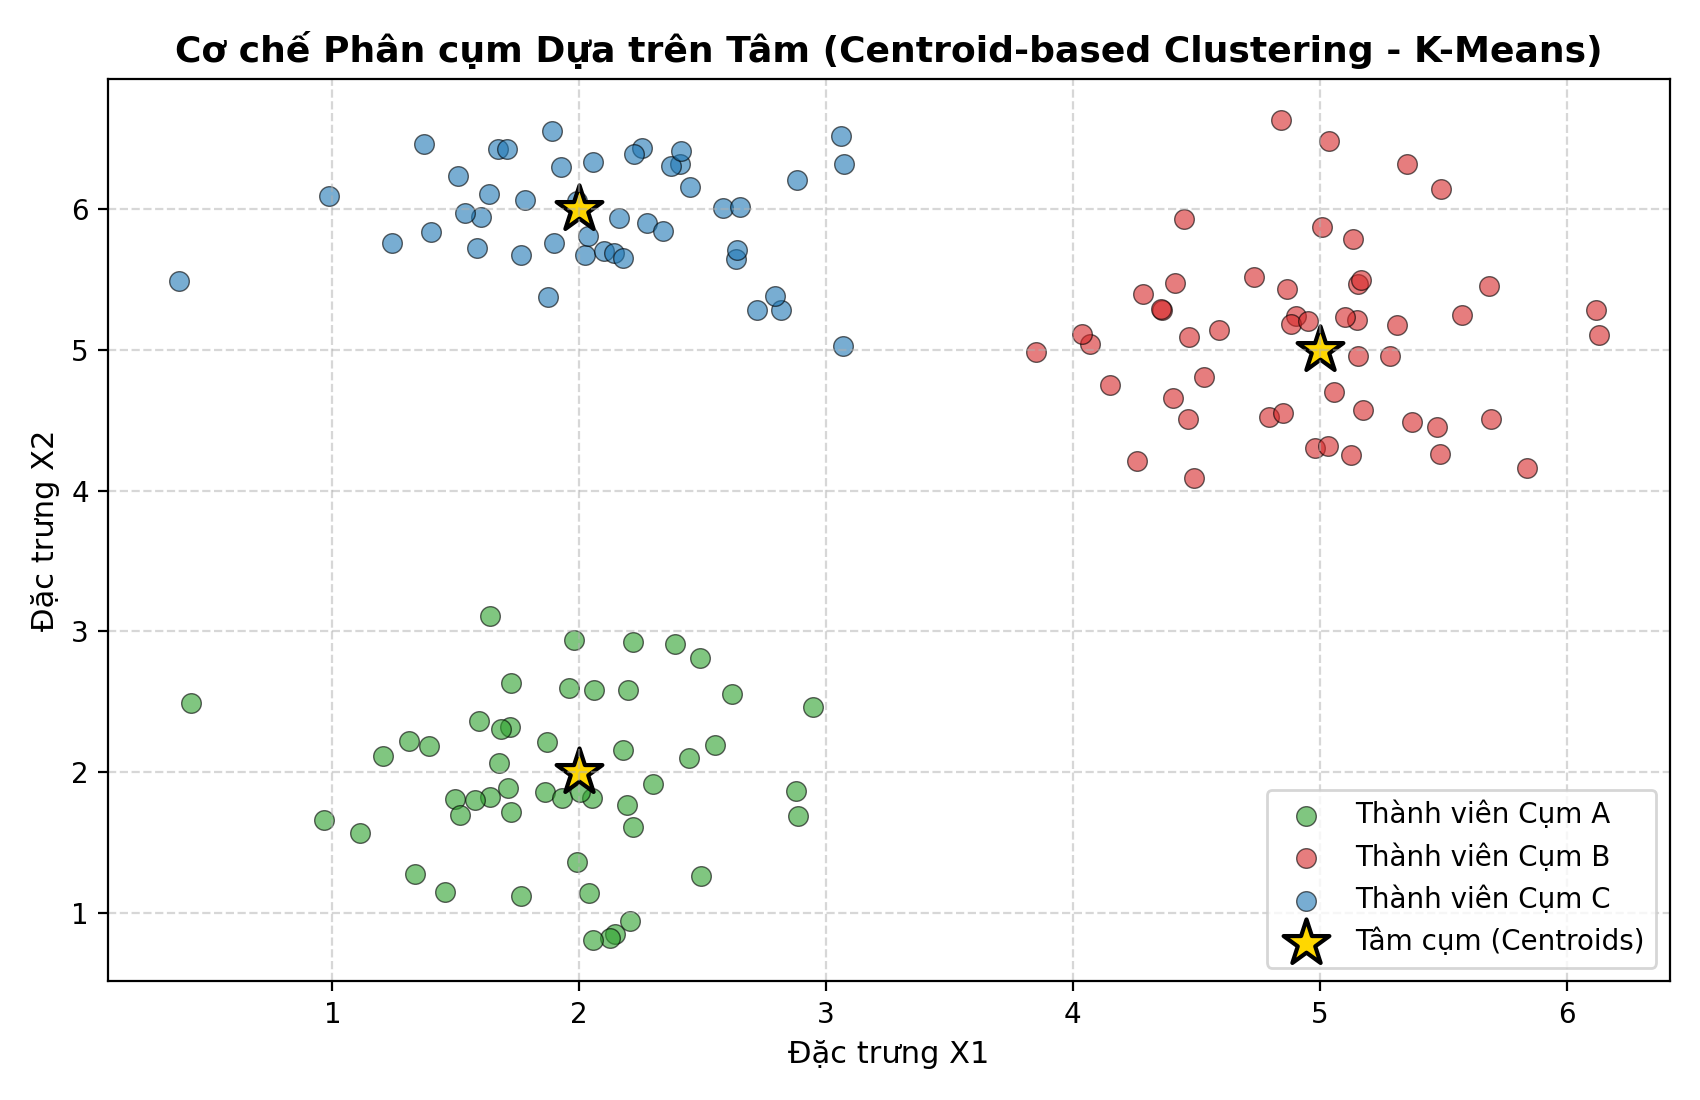
\includegraphics[width=0.95\linewidth,height=0.62\textheight,keepaspectratio]{images/centroid-based-kmeans.png}
      \end{center}
    \end{column}
  \end{columns}
\end{frame}

% Slide 8: K-Means - Giải thích ý nghĩa công thức
\begin{frame}{K-Means: Giải thích Ý nghĩa Toán học \& Trực giác Công thức}
  \footnotesize
  \begin{columns}[T]
    \begin{column}{0.5\textwidth}
      \textbf{1. Ý nghĩa của Hàm WCSS (Inertia):}
      $$J = \sum_{k=1}^K \sum_{x_i \in C_k} \|x_i - \mu_k\|_2^2$$
      \begin{itemize}\setlength{\itemsep}{1.5pt}
        \item Đo \textbf{tổng bình phương độ lệch} của các điểm so với tâm cụm tương ứng.
        \item Tương đương với việc tối thiểu hóa tổng phương sai nội cụm (Compactness).
        \item \textbf{Tại sao tâm là trung bình cộng?} Đạo hàm riêng theo $\mu_k$:
          $$\frac{\partial J}{\partial \mu_k} = -2\sum_{x_i \in C_k} (x_i - \mu_k) = 0 \implies \mu_k = \frac{1}{|C_k|}\sum_{x_i \in C_k} x_i$$
          $\to$ Mean chính là nghiệm cực tiểu giải tích duy nhất cho khoảng cách bình phương Euclidean!
      \end{itemize}
    \end{column}
    \begin{column}{0.5\textwidth}
      \textbf{2. Ý nghĩa Xác suất K-Means++:}
      $$P(x) = \frac{D(x)^2}{\sum_{x' \in \mathcal{X}} D(x')^2}$$
      \begin{itemize}\setlength{\itemsep}{1.5pt}
        \item $D(x)$: Khoảng cách từ điểm $x$ tới tâm gần nhất đã được chọn trước đó.
        \item \textbf{Trực giác:} $D(x)^2$ khuếch đại xác suất chọn các điểm \textbf{ở rất xa các tâm đã có}.
        \item \textbf{Tác dụng sống còn:} Đẩy các tâm khởi tạo tản đều ra toàn không gian, tránh hiện tượng 2 tâm rơi sát nhau trong cùng 1 cụm dày.
        \item \textbf{Cam kết toán học:} Giảm $O(e^K)$ rủi ro cực tiểu cục bộ xuống kỳ vọng đạt cận $O(\log K)$ so với lời giải tối ưu toàn cục.
      \end{itemize}
    \end{column}
  \end{columns}
\end{frame}

% Slide 9: Ví dụ Tính tay K-Means
\begin{frame}{K-Means: Ví dụ Tính tay Chi tiết Từng bước (1 Vòng lặp)}
  \scriptsize
  \textbf{Bài toán mẫu:} Cho 4 quan sát 2 chiều: $A(1, 1), B(2, 1), C(4, 3), D(5, 4)$. Cần phân thành $K=2$ cụm.\\
  \textbf{Khởi tạo:} Chọn tâm ban đầu $\mu_1^{(0)} = A(1, 1)$ và $\mu_2^{(0)} = D(5, 4)$.
  
  \vspace{0.4em}
  \begin{columns}[T]
    \begin{column}{0.5\textwidth}
      \textbf{Bước 1: Tính khoảng cách bình phương \& Gán cụm}
      \begin{itemize}\setlength{\itemsep}{1pt}
        \item Điểm $A(1, 1)$:
          $d^2(A, \mu_1) = 0$; $d^2(A, \mu_2) = (1-5)^2 + (1-4)^2 = 16 + 9 = \mathbf{25} \implies \mathbf{A \in C_1}$.
        \item Điểm $B(2, 1)$:
          $d^2(B, \mu_1) = (2-1)^2 + 0 = \mathbf{1}$; $d^2(B, \mu_2) = 9 + 9 = 18 \implies \mathbf{B \in C_1}$.
        \item Điểm $C(4, 3)$:
          $d^2(C, \mu_1) = 9 + 4 = 13$; $d^2(C, \mu_2) = (4-5)^2 + (3-4)^2 = \mathbf{2} \implies \mathbf{C \in C_2}$.
        \item Điểm $D(5, 4)$:
          $d^2(D, \mu_1) = 16 + 9 = 25$; $d^2(D, \mu_2) = \mathbf{0} \implies \mathbf{D \in C_2}$.
      \end{itemize}
      $\implies$ Phân cụm vòng 1: $C_1 = \{A, B\}$, $C_2 = \{C, D\}$.
    \end{column}
    \begin{column}{0.5\textwidth}
      \textbf{Bước 2: Cập nhật tọa độ tâm cụm mới $\mu^{(1)}$}
      $$\mu_1^{(1)} = \frac{A + B}{2} = \left(\frac{1+2}{2}, \frac{1+1}{2}\right) = \mathbf{(1.5, 1.0)}$$
      $$\mu_2^{(1)} = \frac{C + D}{2} = \left(\frac{4+5}{2}, \frac{3+4}{2}\right) = \mathbf{(4.5, 3.5)}$$
      \vspace{0.2em}
      \textbf{Bước 3: Đánh giá suy giảm của hàm WCSS ($J$)}
      \begin{itemize}\setlength{\itemsep}{1pt}
        \item $J^{(0)} = d^2(A, \mu_1^{(0)}) + d^2(B, \mu_1^{(0)}) + d^2(C, \mu_2^{(0)}) + d^2(D, \mu_2^{(0)}) = 0 + 1 + 2 + 0 = \mathbf{3.0}$.
        \item $J^{(1)} = 2 \times [(0.5)^2 + 0] + 2 \times [(0.5)^2 + (0.5)^2] = 0.5 + 1.0 = \mathbf{1.5}$.
      \end{itemize}
      $\implies$ WCSS giảm từ $3.0 \to 1.5$! Nếu lặp tiếp, gán cụm không đổi $\to$ Hội tụ!
    \end{column}
  \end{columns}
\end{frame}

% Slide 10: Centroid-based - Ứng dụng & Trường hợp Phù hợp
\begin{frame}{Centroid-based: Ứng dụng Thực tế \& Trường hợp Phù hợp}
  \small
  \begin{columns}[T]
    \begin{column}{0.5\textwidth}
      \textbf{1. Ứng dụng Thực tế Đột phá:}
      \begin{itemize}\setlength{\itemsep}{2pt}
        \item \textbf{Phân khúc Khách hàng RFM (E-commerce):}
          Shopee/Tiki nhóm khách hàng theo 3 biến: Recency (ngày mua gần nhất), Frequency (tần suất), Monetary (chi tiêu). Cụm $K=4$: VIP, Khách hàng trung thành, Khách tiềm năng, Khách nguy cơ rời bỏ.
        \item \textbf{Nén Ảnh (Color Quantization):}
          Ảnh RGB 24-bit có $16.7$ triệu màu. K-Means gom các pixel thành $K=16$ hoặc $64$ màu tâm cụm, lưu trữ dạng Palette, giảm $75-85\%$ dung lượng ảnh mà mắt thường khó nhận biết.
        \item \textbf{Tối ưu Vị trí Kho bãi / Trạm sạc EV:}
          Tìm toạ độ tâm cụm $\mu_k$ giảm thiểu tổng quãng đường vận chuyển tới khách hàng.
      \end{itemize}
    \end{column}
    \begin{column}{0.5\textwidth}
      \textbf{2. Cẩm nang Lựa chọn (Khi nào nên dùng?):}
      \begin{itemize}\setlength{\itemsep}{2pt}
        \item \textcolor{darkgreen}{\textbf{NÊN DÙNG KHI:}}
          \begin{itemize}
            \item Dữ liệu quy mô lớn ($N > 10^5 \to 10^7$).
            \item Cụm có hình thái hình cầu lồi (Spherical), kích thước và mật độ các cụm tương đương nhau.
            \item Cần tốc độ huấn luyện nhanh, dễ triển khai lên Production.
          \end{itemize}
        \item \textcolor{crimsonred}{\textbf{KHÔNG NÊN DÙNG KHI:}}
          \begin{itemize}
            \item Cụm có hình dạng phi cầu (hình lưỡi liềm, vành khuyên, xoắn ốc).
            \item Dữ liệu có nhiều ngoại lai (K-Means bị lệch tâm, nên đổi sang \textbf{K-Medoids / PAM}).
            \item Các cụm có mật độ chênh lệch quá lớn.
          \end{itemize}
      \end{itemize}
    \end{column}
  \end{columns}
\end{frame}

% Slide 11: Connectivity-based - Hierarchical
\begin{frame}{3. Connectivity-based: Phân cụm Phân cấp (Hierarchical)}
  \begin{columns}[T]
    \begin{column}{0.55\textwidth}
      \textbf{Hai hướng tiếp cận đối ngẫu:}
      \begin{enumerate}\setlength{\itemsep}{2pt}
        \item \textbf{Agglomerative (Tích tụ / Bottom-Up):}
          \begin{itemize}
            \item Bắt đầu: $N$ cụm đơn lẻ ($N$ lá).
            \item Mỗi bước: Gộp 2 cụm gần nhau nhất.
            \item Kết thúc: 1 siêu cụm duy nhất (Gốc).
          \end{itemize}
        \item \textbf{Divisive (Phân tách / Top-Down):}
          \begin{itemize}
            \item Bắt đầu: 1 cụm tổng thể chứa toàn bộ dữ liệu.
            \item Phân rã đệ quy thành các cụm nhỏ hơn.
          \end{itemize}
      \end{enumerate}
      \textbf{Ưu thế nổi bật:} Không cần chọn trước số lượng cụm $K$ khi dựng cây! Cung cấp bức tranh cấu trúc ở mọi mức độ chi tiết.
    \end{column}
    \begin{column}{0.45\textwidth}
      \begin{center}
        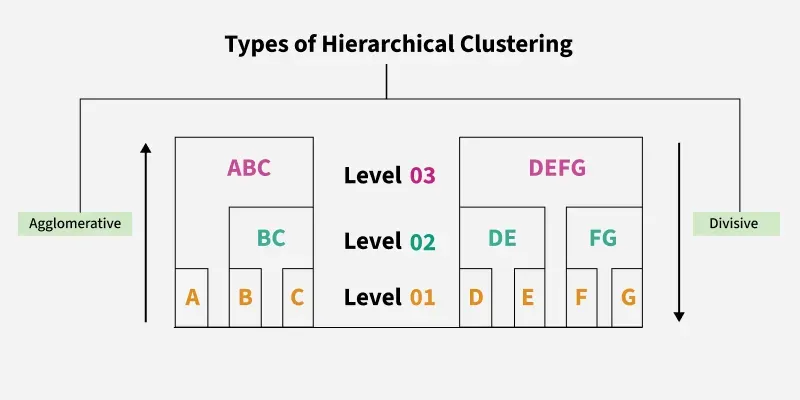
\includegraphics[width=0.95\linewidth,height=0.62\textheight,keepaspectratio]{images/types-of-hierarchical-clustering.png}
      \end{center}
    \end{column}
  \end{columns}
\end{frame}

% Slide 12: Hierarchical - Giải thích ý nghĩa công thức Linkage
\begin{frame}{Hierarchical: Ý nghĩa Toán học \& Trực giác 5 Tiêu chuẩn Linkage}
  \footnotesize
  \begin{columns}[T]
    \begin{column}{0.5\textwidth}
      \textbf{1. Single Linkage (Khoảng cách Tối thiểu):}
      $$D(A, B) = \min_{x \in A, y \in B} d(x, y)$$
      \begin{itemize}\setlength{\itemsep}{1pt}
        \item \textbf{Ý nghĩa:} Gom 2 cụm dựa trên khoảng cách giữa 2 điểm gần nhau nhất (Nearest-neighbor chaining).
        \item \textbf{Điểm yếu chí mạng:} Dễ bị \textbf{Hiện tượng nối chuỗi (Chaining Effect)} -- một cây cầu gồm vài điểm nhiễu có thể nối dính 2 cụm khổng lồ hoàn toàn tách biệt.
      \end{itemize}
      \vspace{0.2em}
      \textbf{2. Complete Linkage (Khoảng cách Tối đa):}
      $$D(A, B) = \max_{x \in A, y \in B} d(x, y)$$
      \begin{itemize}\setlength{\itemsep}{1pt}
        \item \textbf{Ý nghĩa:} Khoảng cách giữa 2 điểm xa nhất. Ép các cụm sáp nhập phải có đường kính bao nhỏ gọn, tạo cụm tròn đặc. Rất nhạy cảm với ngoại lai.
      \end{itemize}
    \end{column}
    \begin{column}{0.5\textwidth}
      \textbf{3. Average Linkage (Trung bình):}
      $$D(A, B) = \frac{1}{|A||B|}\sum_{x \in A}\sum_{y \in B} d(x, y)$$
      \begin{itemize}\setlength{\itemsep}{1pt}
        \item Cân bằng giữa Single và Complete, ít nhạy cảm với nhiễu.
      \end{itemize}
      \vspace{0.2em}
      \textbf{4. Phương pháp Ward (Ward's Minimum Variance):}
      $$\Delta \text{WCSS} = \frac{|A||B|}{|A| + |B|}\|\mu_A - \mu_B\|_2^2$$
      \begin{itemize}\setlength{\itemsep}{1pt}
        \item \textbf{Ý nghĩa:} Chọn sáp nhập 2 cụm làm \textbf{tổng phương sai nội cụm tăng ít nhất}.
        \item \textbf{Khuyến nghị thực tế:} Đây là tiêu chuẩn liên kết \textbf{hiệu quả nhất, phổ biến nhất} trên dữ liệu thực tế!
      \end{itemize}
    \end{column}
  \end{columns}
\end{frame}

% Slide 13: Ví dụ Tính tay Hierarchical
\begin{frame}{Hierarchical: Ví dụ Tính tay Cụm Phân cấp \& Dựng Dendrogram}
  \scriptsize
  \textbf{Bài toán mẫu:} Cho 3 điểm 1 chiều: $A=1.0, B=2.0, C=6.0$. Cần xây dựng cây phân cụm phân cấp Agglomerative.\\
  \textbf{Ma trận khoảng cách ban đầu $D_0$:} $d(A, B) = |1-2| = \mathbf{1.0}$, $d(B, C) = |2-6| = \mathbf{4.0}$, $d(A, C) = |1-6| = \mathbf{5.0}$.
  
  \vspace{0.4em}
  \begin{columns}[T]
    \begin{column}{0.5\textwidth}
      \textbf{Bước 1: Sáp nhập Cặp gần nhau nhất}
      \begin{itemize}\setlength{\itemsep}{1.5pt}
        \item Cặp có khoảng cách nhỏ nhất là $(A, B)$ với $d(A, B) = \mathbf{1.0}$.
        \item Sáp nhập thành cụm mới $C_1 = \{A, B\}$ ở độ cao $h = 1.0$.
      \end{itemize}
      \vspace{0.2em}
      \textbf{Bước 2: Cập nhật khoảng cách từ $\{A, B\}$ tới $C$}
      \begin{itemize}\setlength{\itemsep}{1.5pt}
        \item \textbf{Single Linkage:}
          $$D_{\text{single}}(\{A,B\}, C) = \min(d(A,C), d(B,C)) = \min(5, 4) = \mathbf{4.0}$$
        \item \textbf{Complete Linkage:}
          $$D_{\text{complete}}(\{A,B\}, C) = \max(d(A,C), d(B,C)) = \max(5, 4) = \mathbf{5.0}$$
        \item \textbf{Ward's Method ($\mu_{\{A,B\}} = 1.5, \mu_C = 6$):}
          $$\Delta \text{WCSS} = \frac{2 \times 1}{2 + 1}(1.5 - 6)^2 = \frac{2}{3} \times 20.25 = \mathbf{13.5}$$
      \end{itemize}
    \end{column}
    \begin{column}{0.5\textwidth}
      \textbf{Bước 3: Phân tích Cắt Cây Dendrogram}
      \begin{center}
        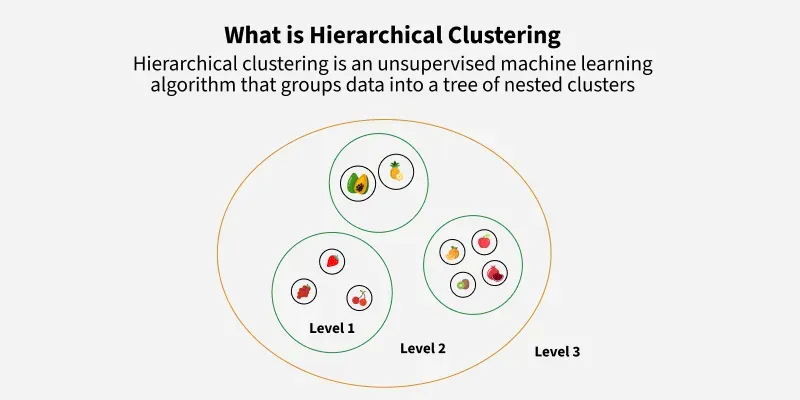
\includegraphics[width=0.92\linewidth,height=0.36\textheight,keepaspectratio]{images/longest-path-dendrogram.png}
      \end{center}
      \textbf{Quy tắc cắt cụm tối ưu:}
      \begin{itemize}\setlength{\itemsep}{1pt}
        \item Nếu muốn $K=2$ cụm: Cắt cây ở độ cao $1.5 < h < 4.0$. Kết quả thu được cụm $\{A, B\}$ và $\{C\}$.
        \item Nhánh dọc từ $1.0 \to 4.0$ (chiều dài $\Delta h = 3.0$) là nhánh dài nhất không bị ngắt quãng $\to$ Khẳng định $K=2$ là cấu trúc tự nhiên mạnh nhất!
      \end{itemize}
    \end{column}
  \end{columns}
\end{frame}

% Slide 14: Connectivity-based - Ứng dụng & Trường hợp Phù hợp
\begin{frame}{Connectivity-based: Ứng dụng Thực tế \& Trường hợp Phù hợp}
  \footnotesize
  \begin{columns}[T]
    \begin{column}{0.5\textwidth}
      \textbf{1. Ứng dụng Thực tế Đột phá:}
      \begin{itemize}\setlength{\itemsep}{2pt}
        \item \textbf{Sinh học \& Phân tích Gen (Bioinformatics):}
          Biểu đồ nhiệt Heatmap kết hợp Dendrogram (Clustered Heatmap) nhóm hàng nghìn gen có mô hình biểu hiện đồng thời, giúp tìm ra các nhóm gen gây ung thư hoặc đáp ứng thuốc.
        \item \textbf{Xây dựng Cây Phân loại Ngành hàng (Taxonomy):}
          Phân cấp đa tầng cho hàng triệu SKU bán lẻ: Ngành hàng $\to$ Danh mục chính $\to$ Tiểu mục $\to$ Sản phẩm.
        \item \textbf{Ngôn ngữ học \& Phát sinh Loài:}
          Xây dựng cây phả hệ tiến hóa sinh vật (Phylogenetic Tree) hoặc phả hệ nguồn gốc các ngữ hệ thế giới.
      \end{itemize}
    \end{column}
    \begin{column}{0.5\textwidth}
      \textbf{2. Cẩm nang Lựa chọn (Khi nào nên dùng?):}
      \begin{itemize}\setlength{\itemsep}{2pt}
        \item \textcolor{darkgreen}{\textbf{NÊN DÙNG KHI:}}
          \begin{itemize}
            \item Nghiệp vụ bắt buộc phải xem xét mối quan hệ phân cấp đa tầng (phòng ban, danh mục).
            \item Kích thước dữ liệu nhỏ đến vừa ($N < 5{,}000$).
            \item Chưa biết số cụm $K$ và muốn linh hoạt thay đổi mức độ gom nhóm bằng cách trượt đường cắt trên Dendrogram.
          \end{itemize}
        \item \textcolor{crimsonred}{\textbf{KHÔNG NÊN DÙNG KHI:}}
          \begin{itemize}
            \item Dữ liệu lớn ($N > 20{,}000$) do bộ nhớ $O(N^2)$ làm tràn RAM và thời gian $O(N^3)$.
            \item Các quyết định sáp nhập sai lầm ở bước đầu không thể sửa đổi (No backtracking).
          \end{itemize}
      \end{itemize}
    \end{column}
  \end{columns}
\end{frame}

% Slide 15: Density-based - DBSCAN
\begin{frame}{4. Density-based: Thuật toán DBSCAN}
  \small
  \begin{columns}[T]
    \begin{column}{0.52\textwidth}
      \textbf{Hai siêu tham số cốt lõi:}
      \begin{itemize}
        \item $\mathbf{\epsilon}$ (Epsilon): Bán kính lân cận vùng khảo sát.
        \item $\mathbf{\text{MinPts}}$: Số lượng mẫu tối thiểu trong bán kính $\epsilon$.
      \end{itemize}
      \vspace{0.2em}
      \textbf{Phân loại 3 nhóm điểm:}
      \begin{itemize}
        \item \textbf{Core Point:} $|N_\epsilon(p)| \ge \text{MinPts}$.
        \item \textbf{Border Point:} $|N_\epsilon(p)| < \text{MinPts}$ nhưng nằm trong bán kính $\epsilon$ của một Core Point.
        \item \textbf{Noise Point:} Không thuộc 2 nhóm trên (gán nhãn \textbf{-1}).
      \end{itemize}
      \vspace{0.2em}
      \textbf{Cơ chế lan truyền cụm:}
      Liên thông mật độ thông qua các chuỗi điểm tiếp cận trực tiếp.
    \end{column}
    \begin{column}{0.48\textwidth}
      \begin{center}
        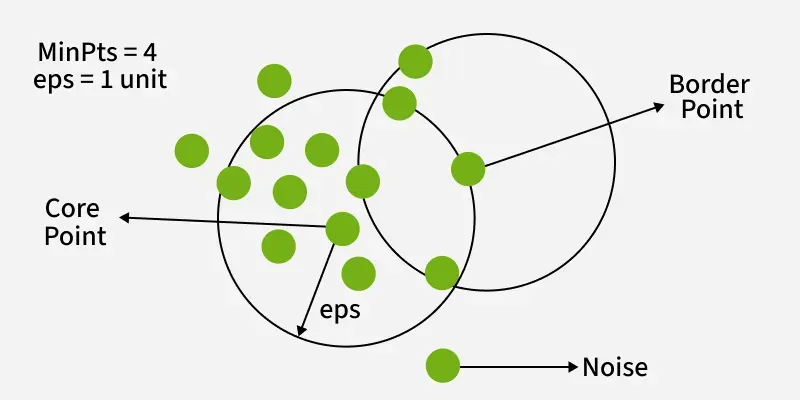
\includegraphics[width=0.95\linewidth,height=0.62\textheight,keepaspectratio]{images/dbscan-core-border-noise.png}
      \end{center}
    \end{column}
  \end{columns}
\end{frame}

% Slide 16: DBSCAN & OPTICS - Giải thích ý nghĩa công thức
\begin{frame}{DBSCAN \& OPTICS: Ý nghĩa Toán học \& Trực giác Mật độ}
  \small
  \begin{columns}[T]
    \begin{column}{0.5\textwidth}
      \textbf{1. Ý nghĩa Mật độ Ngưỡng DBSCAN:}
      \begin{itemize}\setlength{\itemsep}{1.5pt}
        \item Vùng lân cận: $N_\varepsilon(p) = \{q \in \mathcal{X} \mid d(p, q) \le \varepsilon\}$.
        \item \textbf{Mật độ tối thiểu được định nghĩa bởi:}
          $$\rho_{\min} = \frac{\text{MinPts}}{V_\varepsilon}, \quad V_\varepsilon \propto \varepsilon^d$$
        \item Một vùng không gian được xem là \textbf{"Cụm"} nếu mật độ thực tế lớn hơn $\rho_{\min}$.
        \item \textbf{Cơ chế miễn nhiễm Outliers:} Những điểm nằm rải rác ở vùng có mật độ $< \rho_{\min}$ lập tức bị cô lập thành Noise (Nhãn $-1$), không làm lệch hình dạng cụm chính.
      \end{itemize}
    \end{column}
    \begin{column}{0.5\textwidth}
      \textbf{2. Ý nghĩa Reachability Distance (OPTICS):}
      $$\text{rd}(p, o) = \max(\text{core-dist}(o), d(o, p))$$
      \begin{itemize}\setlength{\itemsep}{1.5pt}
        \item DBSCAN thất bại khi các cụm có mật độ khác nhau (chỗ quá đặc, chỗ hơi loãng).
        \item OPTICS giải quyết bằng cách \textbf{làm mịn khoảng cách}: Điểm $p$ chỉ có thể được tiếp cận từ $o$ với khoảng cách tối thiểu bằng Core Distance của $o$.
        \item \textbf{Reachability Plot:} Thung lũng biểu thị cụm mật độ cao, đỉnh núi nhô cao biểu thị ranh giới chia cắt cụm hoặc điểm ngoại lai.
      \end{itemize}
    \end{column}
  \end{columns}
\end{frame}

% Slide 17: Ví dụ Tính tay DBSCAN
\begin{frame}{DBSCAN: Ví dụ Tính tay Phân loại Điểm (Core, Border, Noise)}
  \scriptsize
  \textbf{Bài toán mẫu:} Cho 5 điểm trên trục số 1D: $x_1=1.0, x_2=1.8, x_3=2.5, x_4=5.0, x_5=9.0$.\\
  \textbf{Cấu hình siêu tham số:} Bán kính $\varepsilon = 1.0$, Số điểm tối thiểu $\text{MinPts} = 2$.
  
  \vspace{0.4em}
  \begin{columns}[T]
    \begin{column}{0.52\textwidth}
      \textbf{Bước 1: Quét láng giềng $\varepsilon$-neighborhood cho từng điểm}
      \begin{itemize}\setlength{\itemsep}{1.5pt}
        \item Điểm $x_1(1.0)$: $N_{1.0}(x_1) = \{x_1, x_2\}$ vì $|1.0-1.8| = 0.8 \le 1.0$.
          Số láng giềng $= \mathbf{2 \ge \text{MinPts}} \implies \mathbf{Core\ Point}$.
        \item Điểm $x_2(1.8)$: $N_{1.0}(x_2) = \{x_1, x_2, x_3\}$ vì cách $x_1$ 0.8 và $x_3$ 0.7.
          Số láng giềng $= \mathbf{3 \ge \text{MinPts}} \implies \mathbf{Core\ Point}$.
        \item Điểm $x_3(2.5)$: $N_{1.0}(x_3) = \{x_2, x_3\}$ vì $|2.5-1.8| = 0.7 \le 1.0$.
          Số láng giềng $= \mathbf{2 \ge \text{MinPts}} \implies \mathbf{Core\ Point}$.
        \item Điểm $x_4(5.0)$: $N_{1.0}(x_4) = \{x_4\}$ (chỉ có chính nó).
          Số láng giềng $= \mathbf{1 < \text{MinPts}}$ và cách Core gần nhất $x_3$ là $2.5 > \varepsilon \implies \mathbf{Noise\ Point}$.
        \item Điểm $x_5(9.0)$: $N_{1.0}(x_5) = \{x_5\}$.
          Số láng giềng $= \mathbf{1 < \text{MinPts}} \implies \mathbf{Noise\ Point}$.
      \end{itemize}
    \end{column}
    \begin{column}{0.48\textwidth}
      \textbf{Bước 2: Lan truyền tạo cụm \& Gán nhãn}
      \begin{itemize}\setlength{\itemsep}{2pt}
        \item Xuất phát từ Core $x_1$: kết nạp $x_2$.
        \item Từ Core $x_2$: kết nạp tiếp $x_3$.
        \item Cả 3 điểm $x_1, x_2, x_3$ liên thông mật độ với nhau!
      \end{itemize}
      \vspace{0.2em}
      \textbf{Kết quả Phân cụm Hoàn chỉnh:}
      \begin{table}[]
        \centering
        \begin{tabular}{c c l}
          \toprule
          \textbf{Điểm} & \textbf{Vai trò} & \textbf{Nhãn Phân cụm} \\
          \midrule
          $x_1, x_2, x_3$ & Core Point & \textbf{Cụm 1} \\
          $x_4$ & Noise & \textbf{Ngoại lai (Nhãn -1)} \\
          $x_5$ & Noise & \textbf{Ngoại lai (Nhãn -1)} \\
          \bottomrule
        \end{tabular}
      \end{table}
      \textbf{Nhận xét:} DBSCAN tự động tìm ra 1 cụm đặc và đào thải chuẩn xác 2 điểm dị thường $x_4, x_5$!
    \end{column}
  \end{columns}
\end{frame}

% Slide 18: Density-based - Ứng dụng & Trường hợp Phù hợp
\begin{frame}{Density-based: Ứng dụng Thực tế \& Trường hợp Phù hợp}
  \footnotesize
  \begin{columns}[T]
    \begin{column}{0.5\textwidth}
      \textbf{1. Ứng dụng Thực tế Đột phá:}
      \begin{itemize}\setlength{\itemsep}{2pt}
        \item \textbf{Phát hiện Gian lận Thẻ tín dụng \& An ninh mạng:}
          Hành vi tiêu dùng bình thường tạo thành các cụm dày đặc. Các giao dịch rửa tiền hoặc tấn công DDoS rơi vào vùng mật độ cực thấp $\to$ DBSCAN gán nhãn $-1$ (Noise) phát cảnh báo tức thì.
        \item \textbf{Gom cụm GPS Giao thông (Grab, Be, Uber):}
          Gom hàng triệu toạ độ GPS đón/trả khách để phát hiện điểm nóng tắc đường (Traffic Hotspots), đề xuất trạm đón xe mà không bị nhiễu do lỗi sóng GPS làm méo mó.
        \item \textbf{Thiên văn học:} Phát hiện các chùm sao, dải thiên hà xoắn ốc uốn lượn giữa không gian vũ trụ bao la.
      \end{itemize}
    \end{column}
    \begin{column}{0.5\textwidth}
      \textbf{2. Cẩm nang Lựa chọn (Khi nào nên dùng?):}
      \begin{itemize}\setlength{\itemsep}{2pt}
        \item \textcolor{darkgreen}{\textbf{NÊN DÙNG KHI:}}
          \begin{itemize}
            \item Cụm có hình dạng hình học phức tạp, uốn lượn, phi tuyến tính (non-spherical).
            \item Dữ liệu có tỷ lệ ngoại lai và nhiễu cao cần loại bỏ tự động.
            \item Hoàn toàn không biết trước số lượng cụm $K$.
          \end{itemize}
        \item \textcolor{crimsonred}{\textbf{KHÔNG NÊN DÙNG KHI:}}
          \begin{itemize}
            \item Dữ liệu có mật độ các cụm biến thiên mạnh (chuyển sang dùng \textbf{OPTICS} hoặc \textbf{HDBSCAN}).
            \item Không gian số chiều rất lớn ($d > 20$) vì thể tích khối cầu nở ra quá nhanh làm khoảng cách bị bão hòa (Curse of Dimensionality).
          \end{itemize}
      \end{itemize}
    \end{column}
  \end{columns}
\end{frame}

% Slide 19: Distribution-based - GMM & EM
\begin{frame}{5. Distribution-based: Gaussian Mixture Models (GMM)}
  \begin{columns}[T]
    \begin{column}{0.55\textwidth}
      \textbf{Mô hình xác suất tạo sinh (Generative Model):}
      $$p(x) = \sum_{k=1}^K \pi_k \mathcal{N}(x \mid \mu_k, \Sigma_k)$$
      \begin{itemize}\setlength{\itemsep}{1pt}
        \item $\pi_k$: Trọng số thành phần ($\sum \pi_k = 1$).
        \item $\mu_k$: Vector kỳ vọng (tâm cụm).
        \item $\Sigma_k$: Ma trận hiệp phương sai (hình dạng elip).
      \end{itemize}
      \textbf{Phân cụm mềm (Soft Assignment):}
      $$\gamma_{nk} = P(z_{nk}=1 \mid x_n) = \frac{\pi_k \mathcal{N}(x_n \mid \mu_k, \Sigma_k)}{\sum_{j=1}^K \pi_j \mathcal{N}(x_n \mid \mu_j, \Sigma_j)}$$
    \end{column}
    \begin{column}{0.45\textwidth}
      \begin{center}
        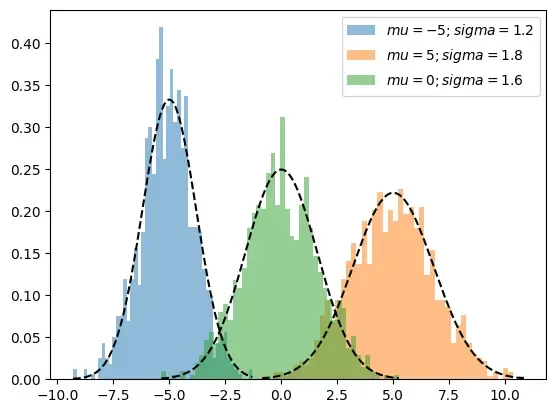
\includegraphics[width=0.92\linewidth,height=0.62\textheight,keepaspectratio]{images/gmm-distribution-concept.png}
      \end{center}
    \end{column}
  \end{columns}
\end{frame}

% Slide 20: Thuật toán EM - Giải thích ý nghĩa công thức
\begin{frame}{Thuật toán EM: Ý nghĩa Toán học \& Trực giác Bước E-step / M-step}
  \small
  \begin{columns}[T]
    \begin{column}{0.5\textwidth}
      \textbf{1. Trực giác Bước E-step (Expectation):}
      $$\gamma_{nk} = \frac{\pi_k \mathcal{N}(x_n \mid \mu_k, \Sigma_k)}{\sum_{j=1}^K \pi_j \mathcal{N}(x_n \mid \mu_j, \Sigma_j)}$$
      \begin{itemize}\setlength{\itemsep}{1.5pt}
        \item Thực chất là áp dụng \textbf{Định lý Bayes}: Tính xác suất hậu nghiệm (Posterior) rằng điểm $x_n$ được sinh ra từ cụm Gaussian thứ $k$.
        \item Không gán nhãn cứng kiểu nhị phân $0/1$, mà phân bổ \textbf{"trách nhiệm mềm"} (ví dụ: $80\%$ thuộc Cụm 1, $20\%$ thuộc Cụm 2).
      \end{itemize}
    \end{column}
    \begin{column}{0.5\textwidth}
      \textbf{2. Trực giác Bước M-step (Maximization):}
      $$\mu_k = \frac{\sum_{n=1}^N \gamma_{nk} x_n}{\sum_{n=1}^N \gamma_{nk}}, \quad N_k = \sum_{n=1}^N \gamma_{nk}$$
      $$\Sigma_k = \frac{1}{N_k}\sum_{n=1}^N \gamma_{nk} (x_n - \mu_k)(x_n - \mu_k)^T$$
      \begin{itemize}\setlength{\itemsep}{1.5pt}
        \item Mỗi điểm dữ liệu đều đóng góp vào việc điều chỉnh toạ độ tâm $\mu_k$ và ma trận xoay $\Sigma_k$ theo đúng tỷ lệ trách nhiệm $\gamma_{nk}$.
        \item \textbf{Bảo đảm toán học:} Giá trị Log-Likelihood $\ln p(\mathcal{X} \mid \theta)$ luôn tăng đơn điệu sau mỗi vòng lặp!
      \end{itemize}
    \end{column}
  \end{columns}
\end{frame}

% Slide 21: Ví dụ Tính tay GMM Bước E-step
\begin{frame}{GMM: Ví dụ Tính tay Bước E-step (Tính Ma trận Trách nhiệm $\gamma$)}
  \scriptsize
  \textbf{Bài toán mẫu:} Cho 2 cụm Gaussian 1D: Cụm 1 $\sim \mathcal{N}(\mu_1=2.0, \sigma_1^2=1.0)$, Cụm 2 $\sim \mathcal{N}(\mu_2=6.0, \sigma_2^2=1.0)$.\\
  Trọng số tiên nghiệm cân bằng: $\pi_1 = \pi_2 = 0.5$. Cần tính trách nhiệm mềm $\gamma_1, \gamma_2$ cho quan sát $x = 3.0$.
  
  \vspace{0.4em}
  \begin{columns}[T]
    \begin{column}{0.52\textwidth}
      \textbf{Bước 1: Tính hàm mật độ xác suất Gaussian $\mathcal{N}(x \mid \mu, \sigma)$}
      Hàm mật độ chuẩn 1D: $\mathcal{N}(x \mid \mu, \sigma) = \frac{1}{\sigma \sqrt{2\pi}} e^{-\frac{(x - \mu)^2}{2\sigma^2}}$.
      Với $\sigma=1.0 \implies \frac{1}{\sqrt{2\pi}} \approx 0.3989$.
      \begin{itemize}\setlength{\itemsep}{2pt}
        \item Đối với Cụm 1 ($\mu_1 = 2.0$):
          $$\mathcal{N}(3.0 \mid 2.0, 1.0) = 0.3989 \times e^{-\frac{(3-2)^2}{2}} = 0.3989 \times e^{-0.5} \approx \mathbf{0.2420}$$
        \item Đối với Cụm 2 ($\mu_2 = 6.0$):
          $$\mathcal{N}(3.0 \mid 6.0, 1.0) = 0.3989 \times e^{-\frac{(3-6)^2}{2}} = 0.3989 \times e^{-4.5} \approx \mathbf{0.0044}$$
      \end{itemize}
    \end{column}
    \begin{column}{0.48\textwidth}
      \textbf{Bước 2: Tính xác suất hậu nghiệm (E-step)}
      Mẫu số tổng hợp:
      $$p(x=3) = \pi_1 \mathcal{N}_1 + \pi_2 \mathcal{N}_2 = 0.5(0.2420) + 0.5(0.0044) = \mathbf{0.1232}$$
      
      Áp dụng định lý Bayes tính trách nhiệm $\gamma$:
      $$\gamma_1 = \frac{0.5 \times 0.2420}{0.1232} = \frac{0.1210}{0.1232} \approx \mathbf{0.982\ (98.2\%)}$$
      $$\gamma_2 = \frac{0.5 \times 0.0044}{0.1232} = \frac{0.0022}{0.1232} \approx \mathbf{0.018\ (1.8\%)}$$
      
      \textbf{Ý nghĩa kết quả:} Điểm $x=3$ thuộc Cụm 1 với độ tin cậy $98.2\%$, và chỉ có $1.8\%$ khả năng thuộc Cụm 2.
    \end{column}
  \end{columns}
\end{frame}

% Slide 22: Distribution-based - Ứng dụng & Trường hợp Phù hợp
\begin{frame}{Distribution-based: Ứng dụng Thực tế \& Trường hợp Phù hợp}
  \small
  \begin{columns}[T]
    \begin{column}{0.5\textwidth}
      \textbf{1. Ứng dụng Thực tế Đột phá:}
      \begin{itemize}\setlength{\itemsep}{2pt}
        \item \textbf{Xử lý Tiếng nói \& Tách Người nói (Speaker Diarization):}
          Tự động xác định "Ai nói khi nào" trong cuộc họp. Các đặc trưng âm phổ MFCC của từng giọng nói được mô hình hóa thành các phân phối Gaussian đa chiều.
        \item \textbf{Phân đoạn Ảnh Y tế (Brain MRI Segmentation):}
          Mô não thực tế có vùng ranh giới chuyển tiếp (Partial Volume Effect) giữa chất xám, chất trắng và dịch não tủy. GMM cung cấp xác suất mềm phản ánh trung thực độ pha trộn mô học.
        \item \textbf{Mô hình hóa Rủi ro Tài chính (Regime Switching):}
          Mô hình hóa thị trường chứng khoán gồm nhiều trạng thái (Thị trường Bò, Gấu, Đi ngang).
      \end{itemize}
    \end{column}
    \begin{column}{0.5\textwidth}
      \textbf{2. Cẩm nang Lựa chọn (Khi nào nên dùng?):}
      \begin{itemize}\setlength{\itemsep}{2pt}
        \item \textcolor{darkgreen}{\textbf{NÊN DÙNG KHI:}}
          \begin{itemize}
            \item Cụm có dạng hình bầu dục (Elip) tự do mọi hướng với kích thước và độ lệch chuẩn khác nhau.
            \item Nghiệp vụ yêu cầu gán mềm (Soft clustering), cần đo lường mức độ không chắc chắn (Uncertainty).
            \item Dữ liệu có sự giao thoa, chồng lấn ranh giới tự nhiên.
          \end{itemize}
        \item \textcolor{crimsonred}{\textbf{KHÔNG NÊN DÙNG KHI:}}
          \begin{itemize}
            \item Cụm có hình phi elip (chữ U, xoắn ốc).
            \item Số chiều $d$ quá lớn khiến ma trận hiệp phương sai $\Sigma$ ($d \times d$) có quá nhiều tham số, dễ bị suy biến (Singular covariance matrix).
          \end{itemize}
      \end{itemize}
    \end{column}
  \end{columns}
\end{frame}

% Slide 23: Fuzzy Clustering - Fuzzy C-Means (FCM)
\begin{frame}{Trường phái Thứ 5: Phân cụm Mờ (Fuzzy C-Means - FCM)}
  \small
  \begin{columns}[T]
    \begin{column}{0.55\textwidth}
      \textbf{Bản chất Phân cụm Mờ (Bezdek, 1981):}
      \begin{itemize}\setlength{\itemsep}{1pt}
        \item Mở rộng mềm từ K-Means, mỗi điểm thuộc về tất cả các cụm với mức độ mờ $u_{ik} \in [0, 1]$ thỏa mãn $\sum_{k=1}^K u_{ik} = 1$.
      \end{itemize}
      \textbf{Hàm mục tiêu mờ ($m > 1$ là tham số mờ hóa):}
      $$J_m = \sum_{i=1}^N \sum_{k=1}^K u_{ik}^m \|x_i - \mu_k\|^2 \to \min$$
      \textbf{Công thức tính độ thuộc $u_{ik}$ \& Tâm $\mu_k$:}
      $$u_{ik} = \frac{1}{\sum_{j=1}^K \left(\frac{\|x_i - \mu_k\|}{\|x_i - \mu_j\|}\right)^{\frac{2}{m-1}}}, \quad \mu_k = \frac{\sum_{i=1}^N u_{ik}^m x_i}{\sum_{i=1}^N u_{ik}^m}$$
    \end{column}
    \begin{column}{0.45\textwidth}
      \textbf{Ví dụ Tính tay FCM với $m=2$:}
      \begin{itemize}\setlength{\itemsep}{1.5pt}\scriptsize
        \item Cho điểm $x=2.0$ giữa 2 tâm $\mu_1=1.0, \mu_2=5.0$.
        \item Khoảng cách: $d_1 = |2-1|=1.0$, $d_2 = |2-5|=3.0$.
        \item Độ thuộc Cụm 1:
          $$u_1 = \frac{1}{\left(\frac{1}{1}\right)^2 + \left(\frac{1}{3}\right)^2} = \frac{1}{1 + \frac{1}{9}} = \mathbf{0.9\ (90\%)}$$
        \item Độ thuộc Cụm 2: $u_2 = 1 - 0.9 = \mathbf{0.1\ (10\%)}$.
      \end{itemize}
      \vspace{0.3em}
      \textbf{Ứng dụng \& Trường hợp phù hợp:}
      Chấm điểm khách hàng đa kênh (Omnichannel), phân tích ranh giới tổn thương mô tế bào bệnh học mà không cần giả định phân phối chuẩn như GMM.
    \end{column}
  \end{columns}
\end{frame}

% Slide 24: Đánh giá mô hình phân cụm
\begin{frame}{6. Đánh giá Chất lượng Phân cụm: Ý nghĩa Công thức}
  \footnotesize
  \begin{columns}[T]
    \begin{column}{0.52\textwidth}
      \textbf{Giải phẫu Hệ số Silhouette ($s \in [-1, 1]$):}
      $$s(i) = \frac{b(i) - a(i)}{\max(a(i), b(i))}$$
      \begin{itemize}\setlength{\itemsep}{1.5pt}
        \item $\mathbf{a(i)}$: Khoảng cách trung bình từ $i$ đến các điểm \textbf{cùng cụm} (Độ gắn kết nội cụm -- Cohesion). Càng nhỏ càng tốt!
        \item $\mathbf{b(i)}$: Khoảng cách trung bình từ $i$ đến các điểm thuộc \textbf{cụm lân cận gần nhất} (Độ tách biệt ngoại cụm -- Separation). Càng lớn càng tốt!
        \item \textbf{Ý nghĩa giá trị $s(i)$:}
          \begin{itemize}
            \item $s \approx +1$: $b(i) \gg a(i) \implies$ Phân cụm rất hoàn hảo!
            \item $s \approx 0$: $a(i) \approx b(i) \implies$ Điểm nằm ngay đường ranh giới.
            \item $s < 0$: $a(i) > b(i) \implies$ Điểm bị gán nhầm cụm!
          \end{itemize}
      \end{itemize}
    \end{column}
    \begin{column}{0.48\textwidth}
      \textbf{Các chỉ số khác:}
      \begin{itemize}\setlength{\itemsep}{2pt}
        \item \textbf{Davies-Bouldin Index (DBI):} Tỷ số giữa độ tản mát nội cụm và khoảng cách tâm. \textbf{Càng nhỏ càng tốt}.
        \item \textbf{Calinski-Harabasz (CH):} Tỷ số phương sai liên cụm / nội cụm. \textbf{Càng lớn càng tốt}.
      \end{itemize}
      \vspace{0.3em}
      \textbf{Khi có nhãn đối chuẩn (External):}
      \begin{itemize}\setlength{\itemsep}{1.5pt}
        \item \textbf{Adjusted Rand Index (ARI $\in [-1, 1]$):} Tỷ lệ cặp điểm xếp đúng, khử yếu tố ngẫu nhiên.
        \item \textbf{NMI ($[0, 1]$):} Tương hỗ thông tin chuẩn hóa.
      \end{itemize}
    \end{column}
  \end{columns}
\end{frame}

% Slide 25: Bảng so sánh tổng kết
\begin{frame}{Bảng So sánh Tổng hợp 5 Trường phái Thuật toán}
  \begin{table}[]
    \tiny
    \centering
    \begin{tabularx}{\textwidth}{l *{5}{>{\raggedright\arraybackslash}X}}
      \toprule
      \textbf{Tiêu chí} & \textbf{K-Means} & \textbf{Hierarchical} & \textbf{DBSCAN} & \textbf{OPTICS} & \textbf{GMM / FCM} \\
      \midrule
      \textbf{Loại phân cụm} & Cứng (Hard) & Cứng (Hard) & Cứng (Hard) & Cứng (Hard) & \textbf{Mềm (Soft)} \\
      \textbf{Cần chọn trước $K$?} & \textbf{Bắt buộc} & Không & Không & Không & \textbf{Bắt buộc} \\
      \textbf{Hình thái cụm} & Hình cầu lồi & Hình cầu / Linh hoạt & \textbf{Bất kỳ (Phi tuyến)} & \textbf{Bất kỳ (Phi tuyến)} & \textbf{Hình Elip tự do} \\
      \textbf{Cụm đa mật độ} & Kém & Trung bình & Kém & \textbf{Rất tốt} & Tốt \\
      \textbf{Xử lý ngoại lai} & Kém (bị kéo tâm) & Kém & \textbf{Tự động lọc} & \textbf{Tự động lọc} & Trung bình \\
      \textbf{Độ phức tạp Time} & $O(N \cdot K \cdot I)$ & $O(N^2 \log N)$ & $O(N \log N) \to O(N^2)$ & $O(N \log N) \to O(N^2)$ & $O(N \cdot K \cdot I \cdot d^3)$ \\
      \textbf{Độ phức tạp Space} & $O(N \cdot d)$ & $O(N^2)$ & $O(N)$ & $O(N)$ & $O(N \cdot d + K \cdot d^2)$ \\
      \textbf{Đầu ra trực quan} & Tâm cụm, Voronoi & Dendrogram & Nhãn cụm phẳng & Reachability Plot & Elip tin cậy \\
      \bottomrule
    \end{tabularx}
  \end{table}
\end{frame}

% Slide 26: Cây quyết định lựa chọn thuật toán
\begin{frame}{Cây Quyết định Lựa chọn Thuật toán trong Thực tế}
  \begin{center}
    \resizebox{0.90\textwidth}{!}{
    \begin{tikzpicture}[
      node distance=1.3cm and 1.2cm,
      box/.style={rectangle, draw=codeblue, fill=codegray, text centered, rounded corners, font=\small\bfseries, minimum height=0.8cm, text width=4.2cm},
      leaf/.style={rectangle, draw=darkgreen, fill=darkgreen!15, text centered, rounded corners, font=\small\bfseries, minimum height=0.7cm, text width=3.0cm},
      arrow/.style={->, >=stealth, thick, color=codeblue}
    ]
      \node[box] (root) {Dữ liệu có nhiều Outlier hoặc hình dạng phi cầu?};
      
      \node[box, below left=of root, xshift=-0.5cm] (density) {Mật độ giữa các cụm có biến thiên lớn không?};
      \node[box, below right=of root, xshift=0.5cm] (normal) {Cần phân cụm mềm hay cần cấu trúc phả hệ?};
      
      \node[leaf, below left=of density, xshift=0.5cm] (dbscan) {DBSCAN};
      \node[leaf, below right=of density, xshift=-0.5cm] (optics) {OPTICS / HDBSCAN};
      
      \node[leaf, below left=of normal, xshift=0.3cm] (gmm) {GMM / FCM (Mềm)};
      \node[leaf, below=of normal] (hier) {Hierarchical};
      \node[leaf, below right=of normal, xshift=-0.3cm] (kmeans) {K-Means++};
      
      \draw[arrow] (root) -- node[above left, font=\scriptsize]{Có} (density);
      \draw[arrow] (root) -- node[above right, font=\scriptsize]{Không (Cụm đều)} (normal);
      
      \draw[arrow] (density) -- node[left, font=\scriptsize]{Mật độ đều} (dbscan);
      \draw[arrow] (density) -- node[right, font=\scriptsize]{Đa mật độ} (optics);
      
      \draw[arrow] (normal) -- node[left, font=\scriptsize]{Xác suất/Mờ} (gmm);
      \draw[arrow] (normal) -- node[font=\scriptsize]{Cây phả hệ} (hier);
      \draw[arrow] (normal) -- node[right, font=\scriptsize]{Tốc độ nhanh} (kmeans);
    \end{tikzpicture}
    }
  \end{center}
\end{frame}

% Slide 27: Cẩm nang Kịch bản Thực tế & Thuật toán Phù hợp
\begin{frame}{Cẩm nang Kịch bản Thực tế: Khi Nào Dùng Thuật Toán Nào?}
  \begin{table}[]
    \tiny
    \centering
    \begin{tabularx}{\textwidth}{p{3.2cm} p{2.4cm} X}
      \toprule
      \textbf{Kịch bản Ứng dụng \& Dữ liệu} & \textbf{Thuật toán Đề xuất} & \textbf{Lý do Kỹ thuật \& Điểm Lưu ý} \\
      \midrule
      \textbf{Phân khúc khách hàng TMĐT} ($N > 10^6$, biến RFM, cụm cầu) & \textbf{K-Means++ / Mini-Batch} & Thời gian chạy siêu nhanh $O(N)$, tâm cụm trực quan giúp ban giám đốc ra quyết định ngay. \\
      \addlinespace
      \textbf{Phát hiện rửa tiền, gian lận} (Nhiều giao dịch bất thường) & \textbf{DBSCAN} & Tự động đào thải ngoại lai thành Noise (nhãn -1) mà không làm lệch kết quả phân tích. \\
      \addlinespace
      \textbf{Điểm nóng giao thông GPS} (Mật độ biến thiên, hình cung đường) & \textbf{OPTICS / HDBSCAN} & Bắt trọn các cung đường uốn lượn và thích ứng các vùng mật độ giao thông chênh lệch. \\
      \addlinespace
      \textbf{Cây danh mục ngành hàng, Phân tích biểu hiện gen} ($N < 5000$) & \textbf{Hierarchical (Ward Linkage)} & Biểu đồ Dendrogram trực quan hóa cấu trúc phả hệ đa cấp; không cần phỏng đoán số cụm $K$. \\
      \addlinespace
      \textbf{Phân đoạn mô não MRI, Tách giọng nói cuộc họp} & \textbf{GMM (EM Algorithm)} & Phân cụm mềm (Soft assignment) định lượng độ không chắc chắn tại các ranh giới mô giao thoa. \\
      \addlinespace
      \textbf{Chấm điểm tín dụng vùng biên, Khách hàng đa kênh} & \textbf{Fuzzy C-Means (FCM)} & Độ thuộc mờ $u_{ik} \in [0,1]$ xử lý xuất sắc các trường hợp khách hàng "nửa nọ nửa kia". \\
      \bottomrule
    \end{tabularx}
  \end{table}
\end{frame}

% Slide 28: Thách thức & Hạn chế trong Phân cụm (GeeksforGeeks)
\begin{frame}{Thách thức \& Giới hạn của Phân cụm Dữ liệu (GeeksforGeeks)}
  \small
  \begin{columns}[T]
    \begin{column}{0.5\textwidth}
      \textbf{1. Xác định số lượng cụm $K$ tối ưu:}
      \begin{itemize}\setlength{\itemsep}{2pt}
        \item Vì không có nhãn đối chuẩn, việc chọn $K$ mang tính chủ quan.
        \item Đòi hỏi kết hợp Elbow, Silhouette và kiến thức nghiệp vụ miền (Domain Knowledge).
      \end{itemize}
      \vspace{0.4em}
      \textbf{2. Độ nhạy cảm với Khởi tạo \& Outliers:}
      \begin{itemize}\setlength{\itemsep}{2pt}
        \item K-Means dễ rơi vào cực tiểu cục bộ nếu không dùng K-Means++.
        \item Ngoại lai có thể làm sai lệch hoàn toàn vị trí tâm cụm.
      \end{itemize}
    \end{column}
    \begin{column}{0.5\textwidth}
      \textbf{3. Lời nguyền Số chiều (Curse of Dimensionality):}
      \begin{itemize}\setlength{\itemsep}{2pt}
        \item Khi số chiều $d$ quá lớn, khoảng cách giữa các cặp điểm đều tiến về một giá trị tương đương (Distance Concentration).
        \item \textit{Giải pháp:} Cần giảm chiều bằng PCA/t-SNE trước khi gom cụm.
      \end{itemize}
      \vspace{0.4em}
      \textbf{4. Chi phí Tính toán trên Big Data:}
      \begin{itemize}\setlength{\itemsep}{2pt}
        \item Hierarchical ($O(N^2)$ bộ nhớ) bất khả thi khi $N > 20{,}000$.
        \item Cần chuyển sang Mini-Batch K-Means hoặc BIRCH.
      \end{itemize}
    \end{column}
  \end{columns}
\end{frame}

% Slide 29: Tổng kết & Thực hành
\begin{frame}{Tổng kết \& Lộ trình Thực hành Lab}
  \begin{columns}[T]
    \begin{column}{0.5\textwidth}
      \textbf{Tóm tắt bài học:}
      \begin{itemize}\setlength{\itemsep}{2pt}
        \item Phân cụm là công cụ khám phá cấu trúc tự nhiên mạnh mẽ nhất của Khoa học Dữ liệu.
        \item Không có một thuật toán duy nhất tối ưu cho mọi bài toán (\textit{No Free Lunch Theorem}).
        \item Lựa chọn thuật toán phụ thuộc chặt chẽ vào:
          \begin{itemize}\setlength{\itemsep}{1pt}
            \item Kích thước dữ liệu $N$ (Scale).
            \item Hình thái hình học của cụm (Cầu vs Phi tuyến).
            \item Tỷ lệ nhiễu và ngoại lai.
            \item Yêu cầu bài toán kinh doanh (cứng hay mềm).
          \end{itemize}
      \end{itemize}
    \end{column}
    \begin{column}{0.5\textwidth}
      \textbf{Nội dung Thực hành trong Notebook:}
      \begin{enumerate}\setlength{\itemsep}{2pt}
        \item \textbf{Bài tập tính tay (Hand Calculations):}
          \begin{itemize}
            \item 1 vòng lặp K-Means trên tập số liệu mẫu.
            \item Sáp nhập Single/Complete Linkage.
            \item Phân loại Core/Border/Noise trong DBSCAN.
            \item 1 chu kỳ E-step \& M-step trong GMM.
          \end{itemize}
        \item \textbf{Bài tập Điền khuyết Code (Fill-in-the-Blank):}
          \begin{itemize}
            \item Hoàn thiện code Scikit-Learn.
            \item Tự động chấm điểm (Assert test).
          \end{itemize}
      \end{enumerate}
    \end{column}
  \end{columns}
\end{frame}

\end{document}
